\documentclass[tikz,border=8pt]{standalone}
\usepackage{tikz}
\usepackage{pgfplots}
\usepackage{amsmath, amssymb}

\pgfplotsset{compat=1.18}

\begin{document}

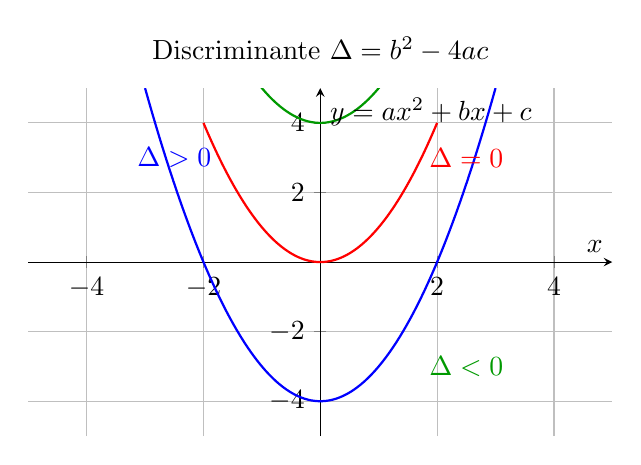
\begin{tikzpicture}[scale=1.0]

  \begin{axis}[
    axis lines = middle,
    xlabel = {$x$},
    ylabel = {$y = ax^2 + bx + c$},
    title = {Discriminante $\Delta = b^2 - 4ac$},
    xmin = -5, xmax = 5,
    ymin = -5, ymax = 5,
    xtick = {-4,-2,0,2,4},
    ytick = {-4,-2,0,2,4},
    grid = major,
    width = 9cm,
    height = 6cm,
  ]

    % Δ > 0: dos raíces (corta eje X en 2 puntos)
    \addplot[blue, thick, domain=-3:3, samples=100] {x^2 - 4};
    \node[blue] at (axis cs:-2.5, 3) {$\Delta > 0$};

    % Δ = 0: una raíz doble (tangente al eje X)
    \addplot[red, thick, domain=-2:2, samples=100] {x^2};
    \node[red] at (axis cs:2.5, 3) {$\Delta = 0$};

    % Δ < 0: sin raíces reales (no corta eje X)
    \addplot[green!60!black, thick, domain=-3:3, samples=100] {x^2 + 4};
    \node[green!60!black] at (axis cs:2.5, -3) {$\Delta < 0$};

  \end{axis}

\end{tikzpicture}

\end{document}
